
%%%%%%%%%%%%%%%%%%
%%%%%%%%%%%%%%%%%%
\begin{frame}
\shiftedframetitle{5. Conclusions}
\vspace{1cm}
\begin{block}{Discontinuities on the subdomain's interface}
\begin{itemize}
\item discontinuities are more prominent in the subcritical case (unsuccessful OpenFOAM-OpenFOAM subcritical case)
\item grid resolution has influence on the discontinuities
\item "simple" mapping techniques (e.g.~velocity mapping)
\item omission of viscosity terms in \textit{SWE solver}
\end{itemize}
\end{block}
\vspace{1cm}
\begin{block}{preCICE across 2D and 3D domains}
\begin{itemize}
\item It is possible to couple subdomains with solvers on different dimensions with preCICE
\item It is possible to extend the SWE-NS models outside the OpenFOAM framework
\end{itemize}

\end{block}


\end{frame}




%\vspace{-2mm}
%{\large Unidirectional Cases}\\
%\begin{multicols}{2}
%\begin{itemize}
%\setlength\itemsep{2em}
%\item \myTUMgreen{2D SWE} domain $\leftrightarrow$ \myTUMgreen{3D interFOAM } domain
%\item fit \myTUMgreen{Fluid-Fluid adapter} preCICE
%\item \myTUMgreen{Exchange} of variables
%\begin{itemize}
%\setlength\itemsep{1em}
%\vspace{5pt}
%\item discharges $hu, hv$
%\item height $h$
%\item volume indicator $\alpha$
%\item \myTUMgreen{BCs} $->$ Dirchlet? Neumann? Robin?
%\end{itemize}
%\end{itemize}
%
%\vfill\columnbreak
%
%\begin{figure}
%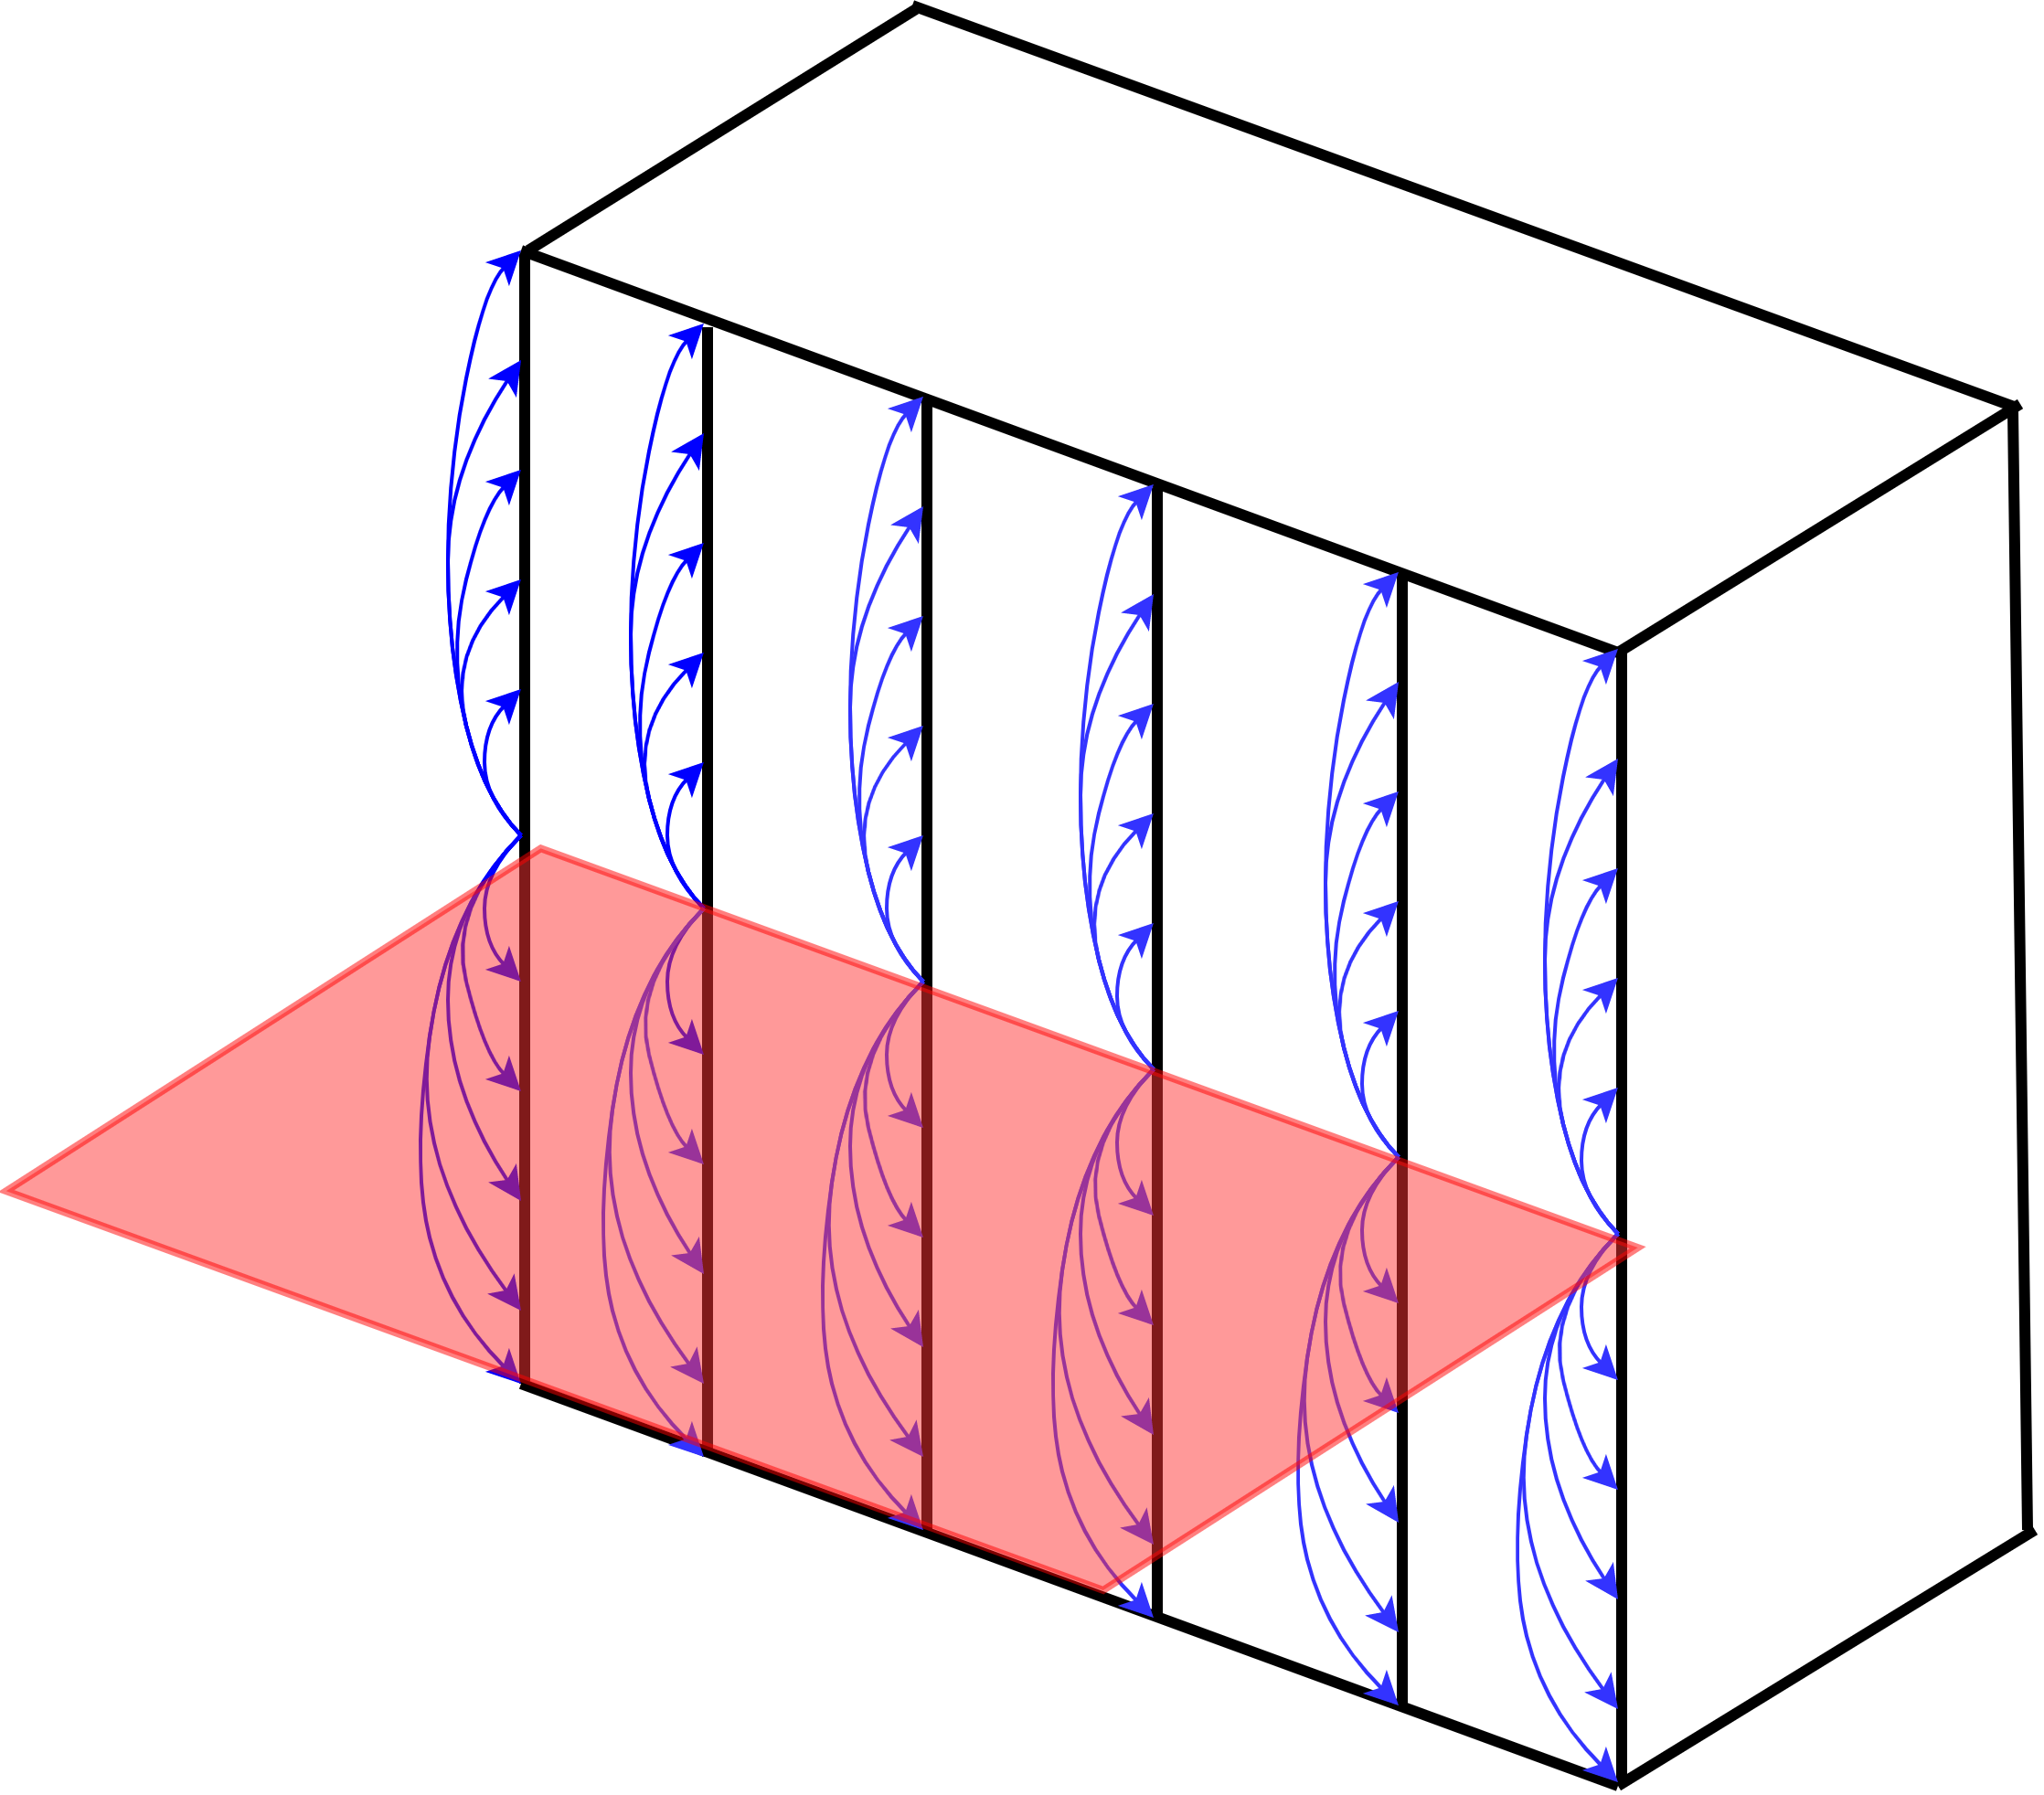
\includegraphics[scale=0.4]{./Resources/Images/mapping23.png}
%\\
%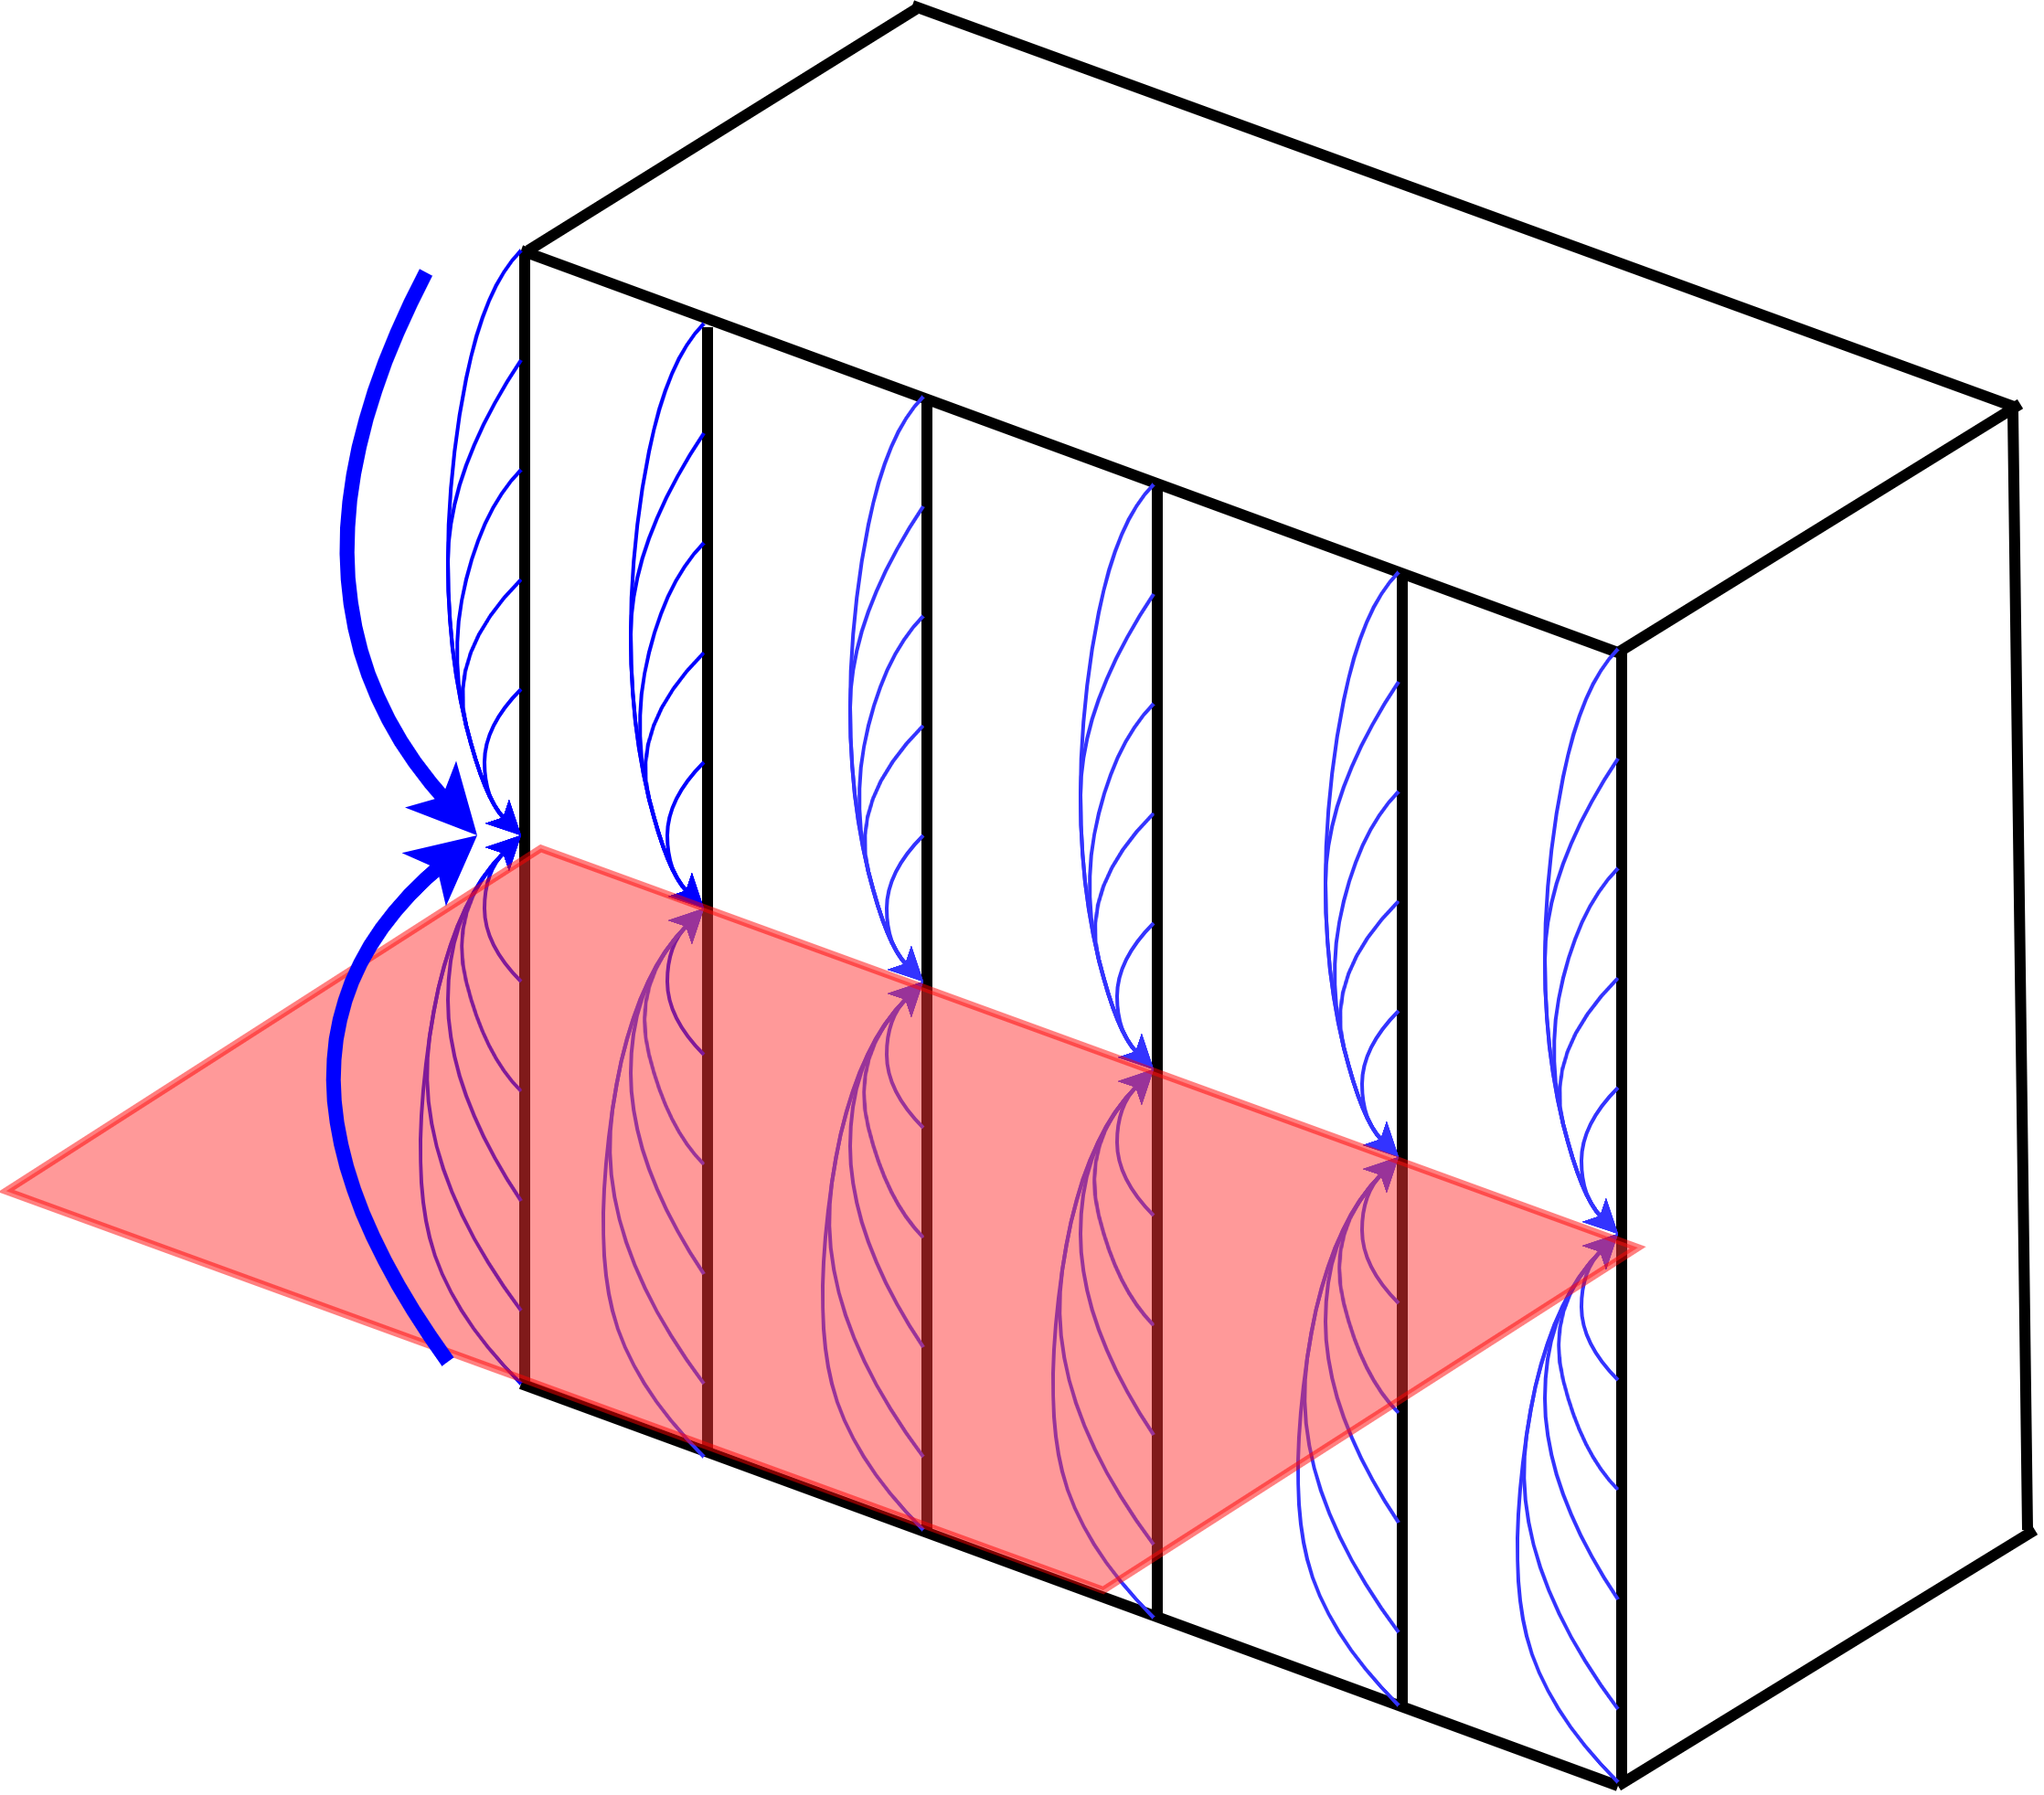
\includegraphics[scale=0.4]{./Resources/Images/mapping32.png}
%
%%\caption<1>{mapping $2D$ to $3D$}
%%\caption<2>{mapping $3D$ to $2D$}
%\end{figure}
%
%\end{multicols}

%%%%%%%%%%%%%%%%%%
%%%%%%%%%%%%%%%%%%
\begin{frame}
\shiftedframetitle{5. Future Work}

\begin{itemize}
\item[]
\begin{exampleblock}{Include viscosity terms }
\textit{SWE solver} omits viscosity, while \textit{interFoam} does consider them.  
\end{exampleblock}
\item[]

\begin{exampleblock}{Mapping with different resolutions}
Currently, mapping between \textit{SWE solver} and \textit{interFoam} is done at a common edge/face with same resolution
\end{exampleblock}
\item[]

\begin{exampleblock}{Implicit coupling}
\textit{SWE solver} and \textit{interFoam} were coupled using explicit coupling from preCICE
\end{exampleblock}
\item[]

\begin{exampleblock}{Add source terms}
Seafloor profiles were not considered in \textit{SWE solver}
\end{exampleblock}
\item[]

\begin{exampleblock}{Try out different mapping algorithms}
Adapter in \textit{SWE solver}  allows to easily add or modify mapping algorithms 
\end{exampleblock}


\end{itemize}


\end{frame}



%\vspace{-2mm}
%{\large Bidirectional $3D$}\\
%\begin{multicols}{2}
%\begin{itemize}
%\setlength\itemsep{2em}
%\item 3D interFOAM  \textit{left} $\leftrightarrow$ \textit{right} domains
%\item fit \myTUMgreen{Fluid-Fluid adapter} preCICE
%\item \myTUMgreen{Exchange} of variables
%\begin{itemize}
%\setlength\itemsep{1em}
%\vspace{5pt}
%\item discharges $hu, hv$
%\item height $h$
%\item volume indicator $\alpha$
%\item \myTUMgreen{BCs} $->$ Dirchlet? Neumann? Robin?
%\end{itemize}
%\end{itemize}
%
%\vfill\columnbreak
%
%\begin{figure}
%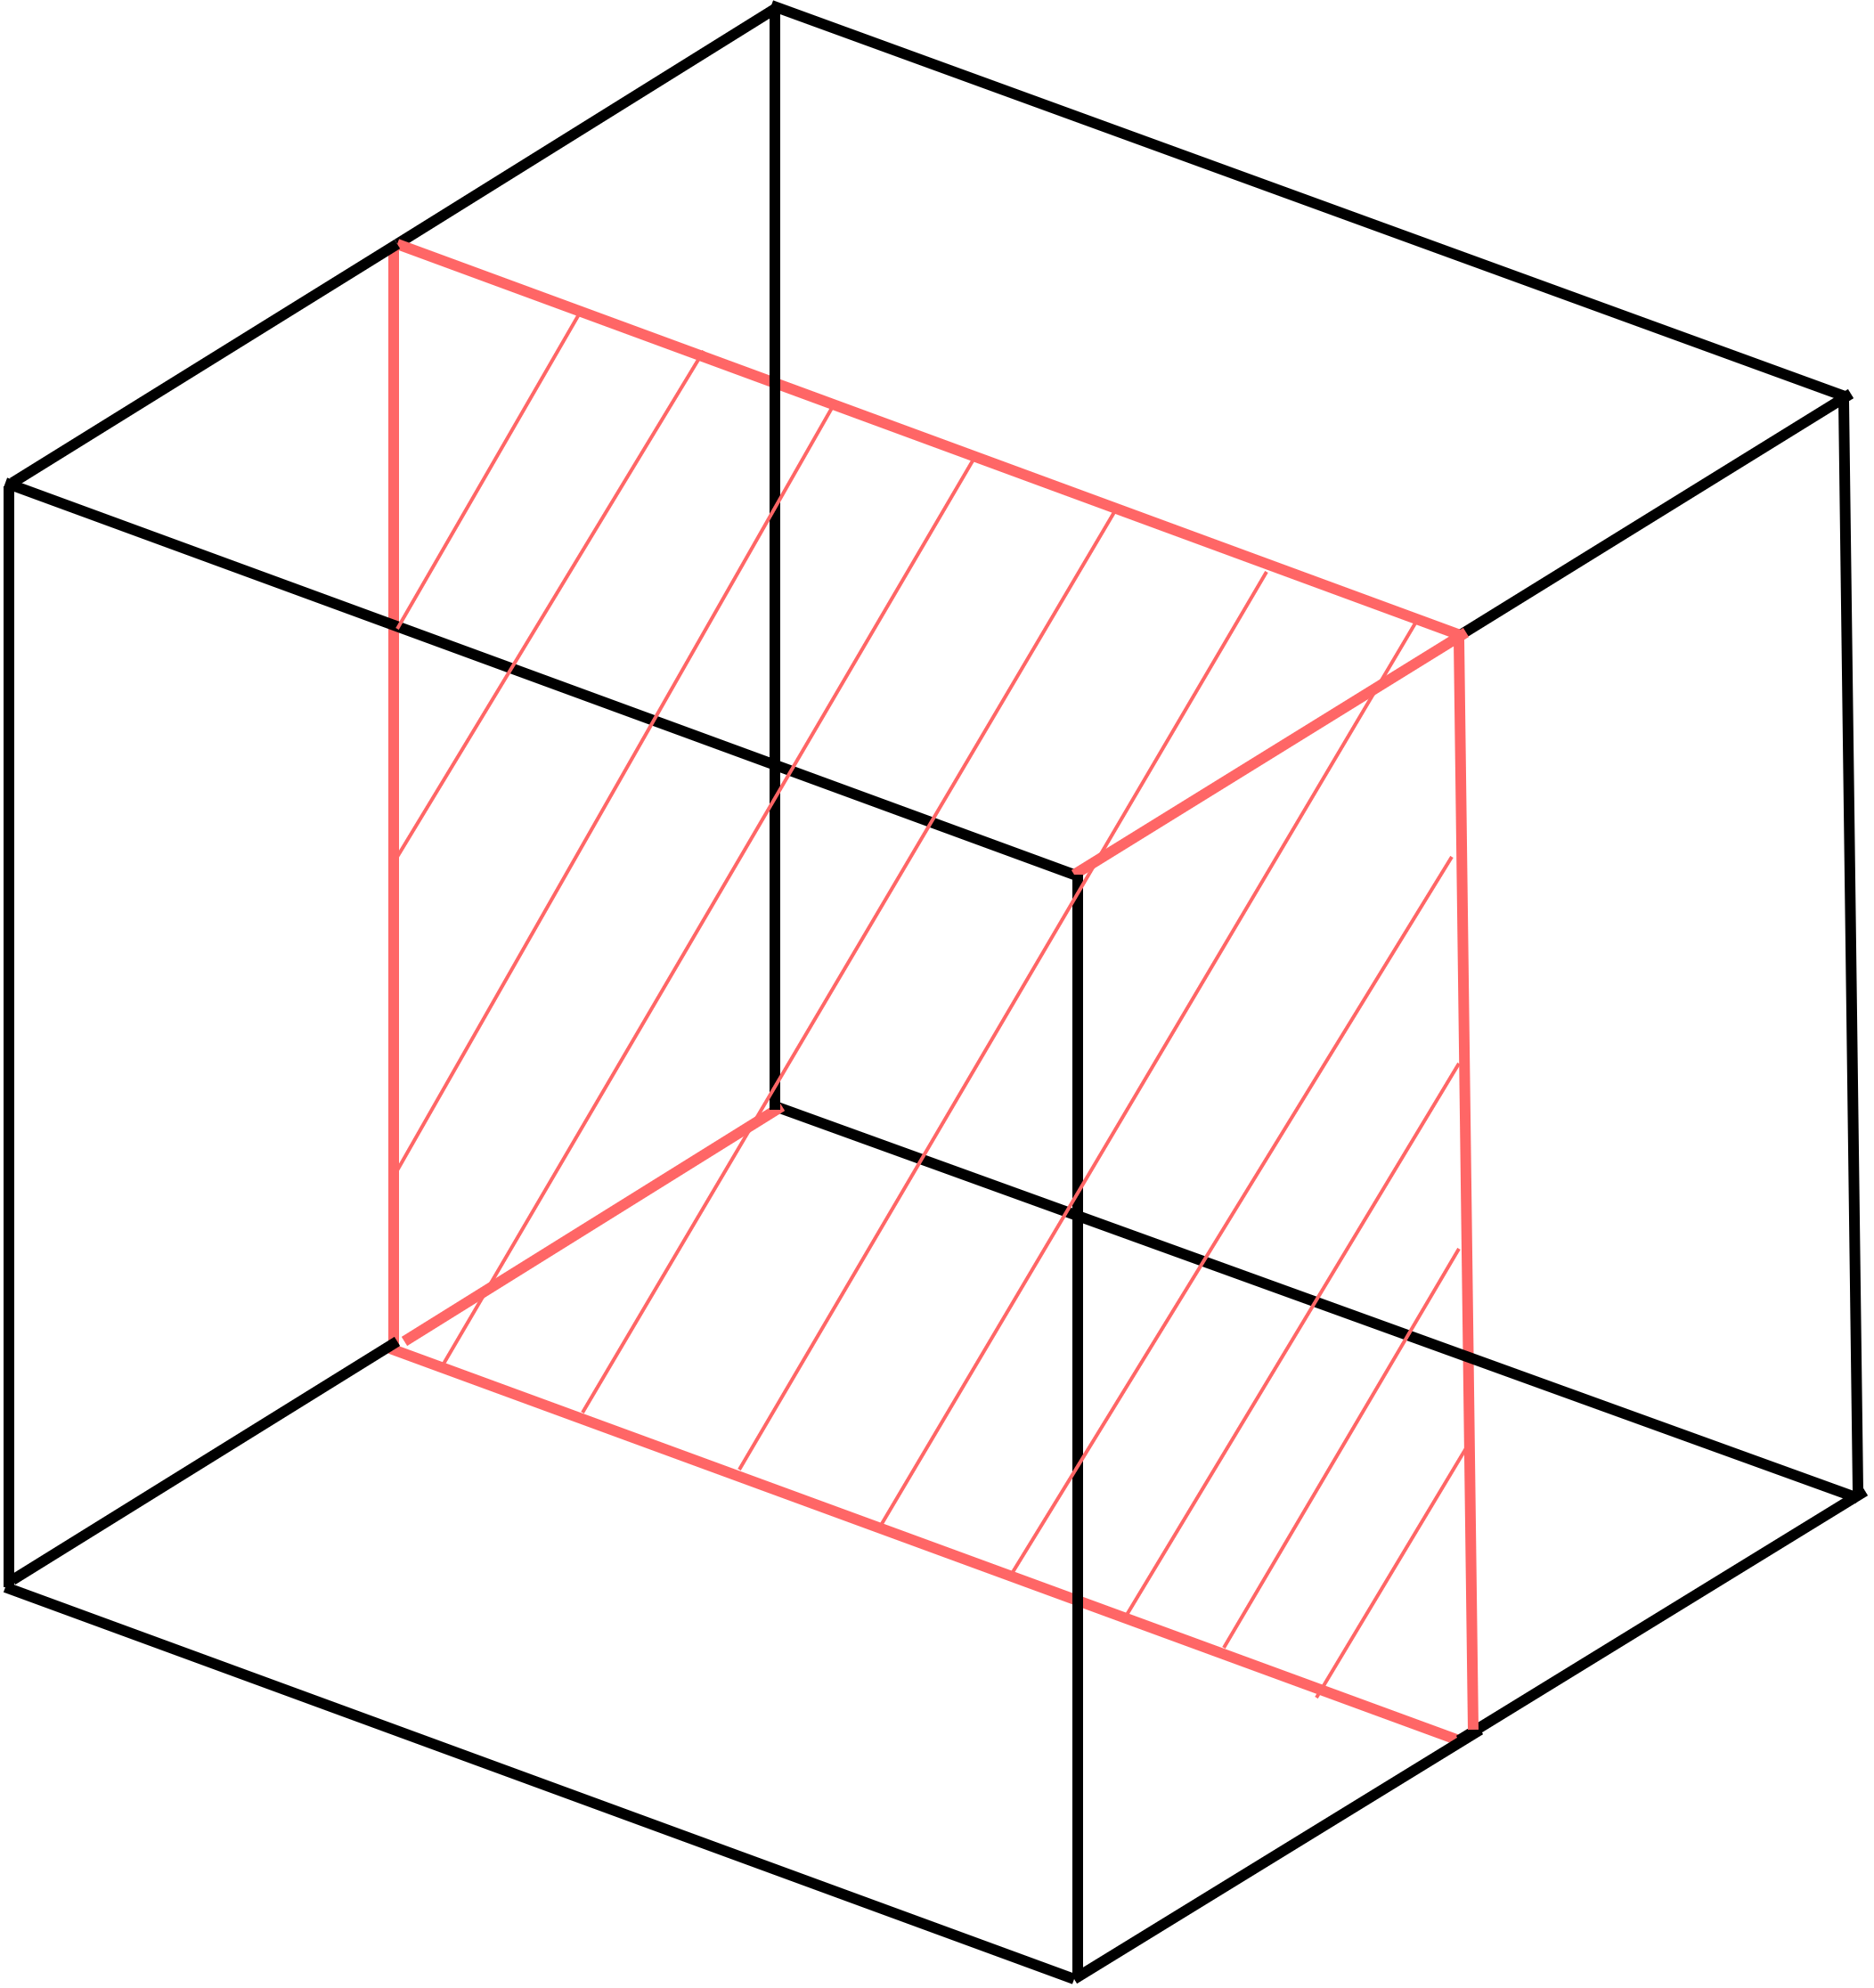
\includegraphics[scale=0.5]{./Resources/Images/mapping33.png}
%%\caption<1>{mapping $2D$ to $3D$}
%%\caption<2>{mapping $3D$ to $2D$}
%\end{figure}
%
%\end{multicols}


%%%%%%%%%%%%%%%%%%%%
%%% Folie: Farben %%
%%%%%%%%%%%%%%%%%%%%
%\begin{frame}
%    \shiftedframetitle{Farben}
%
%Als erstes soll mit schwarz und weiß gearbeitet werden.\newline
%Für Aufwändigere Darstellungen sind Farben mit Bedacht und in möglichst
%geringem Umfang einzusetzen.
%
%In diesem Folienmaster ist die Farbpalette festgelegt.
%
%{
%    \renewcommand{\arraystretch}{1.2} % skaliert die Tabellen mit Farbfeldern
%
%    Zuerst mit den Primärfarben arbeiten.
%
%    \setlength{\fboxsep}{-1pt} \setlength{\fboxrule}{1pt} % fbox/framebox konfigurieren
%
%    \vspace*{-5mm}
%    \begin{tabularx}{\textwidth}{@{} l @{\hspace{4mm}} l @{\hspace{4mm}} l}
%        \crule[TUMBlau]{24mm}{6mm}
%        & \crule[black]{24mm}{6mm}
%        & \fbox{\crule[white]{24mm}{6mm}}
%    \end{tabularx}
%
%    \vspace*{-5mm}
%    Für z.B. komplexe Diagramme stehen noch Sekundärfarben zur Verfügung.
%
%    \vspace*{-5mm}
%    \begin{tabularx}{\textwidth}{@{} l @{\hspace{4mm}} l @{\hspace{4mm}} l @{\hspace{4mm}} l}
%        \crule[TUMBlauDunkel]{24mm}{6mm}
%        & \crule[TUMBlauMittel]{24mm}{6mm}
%        & \crule[TUMBlauHell]{24mm}{6mm}
%        & \crule[TUMGrau]{24mm}{6mm}
%    \end{tabularx}
%
%    \vspace*{-5mm}
%    Bei weiterer Komplexität oder zusätzlichen Markierungen:
%
%    \vspace*{-5mm}
%    \begin{tabularx}{\textwidth}{@{} l @{\hspace{4mm}} l @{\hspace{4mm}} l }
%        \crule[TUMOrange]{24mm}{6mm}
%        & \crule[TUMGruen]{24mm}{6mm}
%        & \crule[TUMElfenbein]{24mm}{6mm}
%    \end{tabularx}
%}
%
%\end{frame}
%\clearpage
%
%
%%%%%%%%%%%%%%%%%%%
%%% Folie: Texte %%
%%%%%%%%%%%%%%%%%%%
%\begin{frame}
%    \shiftedframetitle{Texte}
%
%Kurze und knappe Texte, Fließtexte linksbündig, kein Blocksatz \\[\baselineskip]
%
%Beispiel:\newline
%Tem soluptam, nisi as verum ereprehendam at acculpa quidisq uissit volupta
%tusdant utem as etur, odi odis es doluptiae dem nimaion con nossinctenis pora
%quam voloria consenimus blabore everfer epeliquo maio etur.
%
%\end{frame}
%\clearpage
%
%
%
%
%%%%%%%%%%%%%%%%%%%%%%%%%%%%%%%
%% Folie: Bilder - Allgemein %%
%%%%%%%%%%%%%%%%%%%%%%%%%%%%%%%
%\begin{frame}
%    \shiftedframetitle{Bilder -- Allgemein}
%
%schlichte Darstellung von Informationen \\[\baselineskip]
%
%reduzierte Farben \\[\baselineskip]
%
%Rahmen und Überlagerungen nach Möglichkeit vermeiden \\[\baselineskip]
%
%
%\end{frame}
%\clearpage
%
%
%%%%%%%%%%%%%%%%%%%%%%%%%%
%% Folie: Bilder - Zwei %%
%%%%%%%%%%%%%%%%%%%%%%%%%%
%\begin{frame}
%    \shiftedframetitle{Bilder}
%
%Bildbeschreibung\newline
%oberer Bildrand: Begrenzung durch Text\\[\baselineskip]
%
%\mbox{
\includegraphics[height=.5\paperheight, trim=0cm 14cm 0cm 0cm, clip=true]{./Resources/Images/SternenhimmelHochkant.jpg}}%
%\hspace{6.5mm}%
%\mbox{
\includegraphics[height=.5\paperheight, trim=0cm 14cm 0cm 0cm, clip=true]{./Resources/Images/SternenhimmelHochkant.jpg}}
%
%\end{frame}
%\clearpage
%
%
%%%%%%%%%%%%%%%%%%%%%%%%%%%%%%%%%%%%%%%%
%% Folie: Bilder - Zweispaltige Seite %%
%%%%%%%%%%%%%%%%%%%%%%%%%%%%%%%%%%%%%%%%
%\begin{frame}
%    \shiftedframetitle{Bilder}
%
%\begin{multicols}{2}
%    \textbf{Überschrift 2}\newline
%    Hier steht ein einleitender oder beschreibender Fließtext und nach Wunsch
%    eine Aufzählung.
%
%    Punkt 1
%
%    Punkt 2
%
%    Punkt 3
%
%    Punkt 4
%    \vfill\columnbreak
%    
\includegraphics[width=\columnwidth, height=.7\textheight]{./Resources/Images/SternenhimmelHochkant.jpg}%
%\end{multicols}
%
%\end{frame}
%\clearpage
%
%
%%%%%%%%%%%%%%%%%%%%%%%%%%%%%%%
%% Folie: Bilder - Textbreit %%
%%%%%%%%%%%%%%%%%%%%%%%%%%%%%%%
%\begin{frame}
%    \shiftedframetitle{Bilder}
%
%Bildbeschreibung\newline
%oberer Bildrand: Begrenzung durch Text\\[\baselineskip]
%
%
\includegraphics[width=\textwidth, height=.55\textheight]{./Resources/Images/SternenhimmelQuer.jpg}%
%
%\end{frame}
%\clearpage
%
%%%%%%%%%%%%%%%%%%%%%%%%%%%%%%%%%%%%%%%%%%%%%%%%%%
%% Folie: Bilder - seitenbreit mit Beschreibung %%
%%%%%%%%%%%%%%%%%%%%%%%%%%%%%%%%%%%%%%%%%%%%%%%%%%
%\begin{frame}
%    \shiftedframetitle{Bilder}
%
%    Bildbeschreibung\newline
%    oberer Bildrand: Begrenzung durch Text
%
%\vspace*{-3mm}
%\begin{minipage}[t][0cm]{\paperwidth}%
%\hspace*{-\PraesentationSeitenrand}%
%
\includegraphics[width=\paperwidth]{./Resources/Images/SternenhimmelQuer.jpg}
%\end{minipage}
%
%\end{frame}
%\clearpage
%
%%%%%%%%%%%%%%%%%%%%%%%%%%%%%%%%%%%%%%%%%%%%%%%%%%%%%
%% Folie: Nicht Format füllende Bilder %%
%%%%%%%%%%%%%%%%%%%%%%%%%%%%%%%%%%%%%%%%%%%%%%%%%%%%%
%\begin{frame}
%    \shiftedframetitle{Nicht Format füllende Bilder}
%
%    Weißer bzw. transparenter Hintergrund\newline
%    mit genug Freiraum anordnen
%
%
%\begin{textblock*}{0.4\paperwidth}[0,1](0cm, \textheight - \PraesentationSeitenrand)%
%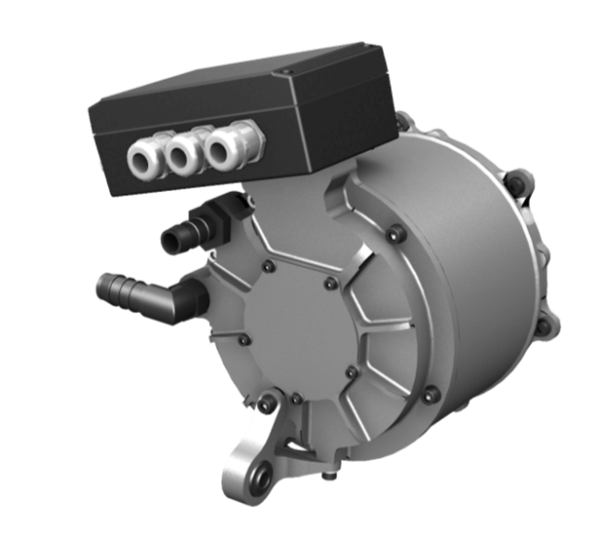
\includegraphics[width=0.4\paperwidth]{./Resources/Presentation/Images/Motor.png}
%\end{textblock*}
%
%\begin{textblock*}{0.6\paperwidth}[1,1](\textwidth + \PraesentationSeitenrand, \textheight - \PraesentationSeitenrand)%
%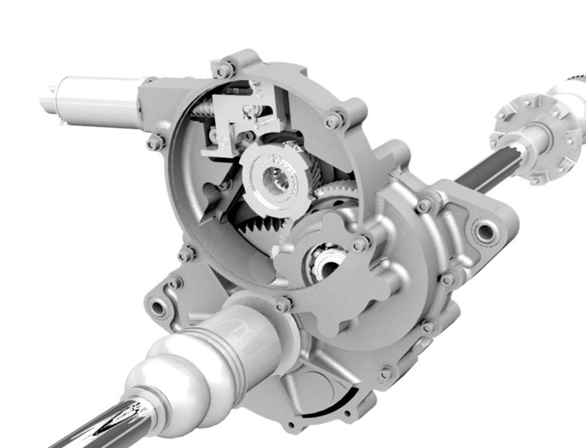
\includegraphics[width=0.6\paperwidth]{./Resources/Presentation/Images/Getriebe.png}
%\end{textblock*}
%
%\end{frame}
%\clearpage
%
%
%%%%%%%%%%%%%%%%%%%%%%%%%%%%%%%%%%%
%% Folie: Bilder - formatfüllend %%
%%%%%%%%%%%%%%%%%%%%%%%%%%%%%%%%%%%
%\begin{frame}
%    \shiftedframetitle{Bilder Format füllend -- maximale Bildgröße}
%
%\begin{minipage}[t][0cm]{\paperwidth}%
%\hspace*{-\PraesentationSeitenrand}%
%
\includegraphics[width=\textwidth]{./Resources/Images/SternenhimmelQuer.jpg}
%\end{minipage}
%
%\end{frame}
%\clearpage
%
%%%%%%%%%%%%%%%%%%%%%%%%%%%%%%%%%%%%%%%%%%%%%%%%%%%%%%
%%% Folie: Nicht Format füllende Bilder %%
%%%%%%%%%%%%%%%%%%%%%%%%%%%%%%%%%%%%%%%%%%%%%%%%%%%%%%
%\begin{frame}
%    \shiftedframetitle{Nicht Format füllende Bilder}
%
%Alternativ mit formatfüllendem Hintergrund: Weiß 5\% dunkler\newline
%Beschriftungen können zusätzlich neben den Bildern angebracht werden
%
%\begin{textblock*}{\paperwidth}[0,0](0cm, .4\textheight)%
%Bilderklärung
%\end{textblock*}
%
%\begin{textblock*}{\paperwidth}[1,0](\textwidth, .4\textheight)%
%\raggedleft%
%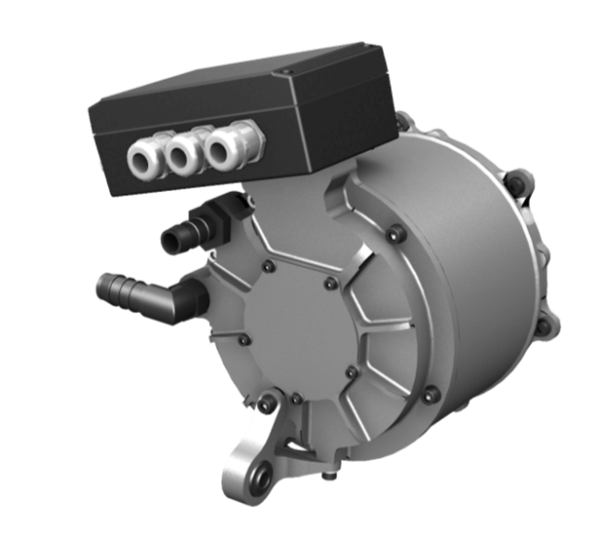
\includegraphics[height=0.5\textheight]{./Resources/Presentation/Images/Motor.png}
%\end{textblock*}
%
%\end{frame}
%\clearpage
%
%
%%%%%%%%%%%%%%%%%%%%%%%%%%%%%%%%%%%%%%%%%%%%%%%%%%%%%
%% Folie: Tabelle - Ohne Rand 					   %%
%%%%%%%%%%%%%%%%%%%%%%%%%%%%%%%%%%%%%%%%%%%%%%%%%%%%%
%\begin{frame}
%    \shiftedframetitle{Tabelle -- Beispiel 1}
%
%Tabelle ohne Farbe und kein Rand \\
%innerer Seitenrand links 0 cm, um Faktor 1,75 skalierte Tabelle (für genug Zeilenabstand)
%
%\raggedright
%{
%    \vspace*{0.3pt}
%    \renewcommand{\arraystretch}{1.75} % skaliert die Tabelle auf die gewünschte Größe
%    \begin{tabularx}{\textwidth}{@{} l @{\hspace{38.7mm}} l}
%        Ø - Strecke & 39 km/Tag (14.360 km/Jahr) \\
%        Ø - Geschwindigkeit & 25 km/h \\
%        Ø - Verfügbare Ladezeit & 22 h/Tag \\
%        Kosten   & Kleinwagen mit Verbrennungsmotor \\
%        Einsatzgebiet   &  Stadt und Umland
%    \end{tabularx}
%}
%\end{frame}
%
%
%%%%%%%%%%%%%%%%%%%%%%%%%%%%%%%%%%%%%%%%%%%%%%%%%%%%%%
%%% Folie: Tabelle - Mit Rand                       %%
%%%%%%%%%%%%%%%%%%%%%%%%%%%%%%%%%%%%%%%%%%%%%%%%%%%%%%
%\begin{frame}
%    \shiftedframetitle{Tabelle -- Beispiel 2}
%
%Tabelle ohne Farbe und mit Rand\\
%automatische Zelleninnenabstände, um Faktor 1,75 skalierte Tabelle (für genug Zeilenabstand)
%
%\raggedright
%{
%    \vspace*{0.3pt}
%    \renewcommand{\arraystretch}{1.75} % skaliert die Tabelle auf die gewünschte Größe
%    \begin{tabularx}{\textwidth}{| l @{\hspace{38.7mm}} | X |}
%        \hline
%        Ø - Strecke & 39 km/Tag (14.360 km/Jahr) \\ \hline
%        Ø - Geschwindigkeit & 25 km/h \\ \hline
%        Ø - Verfügbare Ladezeit & 22 h/Tag \\ \hline
%        Kosten   & Kleinwagen mit Verbrennungsmotor \\ \hline
%        Einsatzgebiet   &  Stadt und Umland \\ \hline
%    \end{tabularx}
%}
%\end{frame}
%
%\clearpage
%
%
%%%%%%%%%%%%%%%%%%%%%%%%%%%%%%%%%%%%%%%%%%%%%%%%%%%%%%
%%% Folie: Diagramme - Beispiel 1                   %%
%%%%%%%%%%%%%%%%%%%%%%%%%%%%%%%%%%%%%%%%%%%%%%%%%%%%%%
%\begin{frame}
%    \shiftedframetitle{Diagramme -- Beispiel 1}
%
%%Nach Möglichkeit linksbündig bleiben \\
%%Unnötige Striche und Balken vermeiden
%
%\begin{center}%
%    \vspace*{-1cm}
%   \begin{tikzpicture}
%        \begin{axis}[
%                % kein Abstand zwischen Balken:
%                xbar=0,
%                draw opacity=0,
%                bar width=14,
%                axis x line=none,
%                axis line style={transparent},
%                every tick/.style={transparent},
%                xmin=0,
%                width=\textwidth,
%                height=.6\textheight,
%                enlarge y limits=0.15,
%                symbolic y coords={Kategorie 4,Kategorie 3,Kategorie 2,Kategorie 1},
%                ytick=data,
%                legend image code/.code={\draw[draw=none] (0cm,-0.12cm) rectangle (0.29cm,0.17cm);}, % Legenden-Symbol
%                legend columns=3,
%                reverse legend,
%                legend style={
%                    fill=none,
%                    draw=none,
%                    /tikz/every odd column/.append style={column sep=0.07cm}, % Abstand zwischen Legenden-Symbol und Text
%                    /tikz/every even column/.append style={column sep=0.8cm} % Abstand zwischen den Legendeneinträgen
%                 },
%                 legend to name=PraesentationDiagrammHorizontalLegende
%            ]
%
%            \addlegendentry{Datenreihe 3}
%            \addlegendentry{Datenreihe 2}
%            \addlegendentry{Datenreihe 1}
%
%            \addplot[color=TUMBlauMittel, fill=TUMBlauMittel] coordinates {
%                (1.2,Kategorie 1)
%                (1.6,Kategorie 2)
%                (2.2,Kategorie 3)
%                (3.4,Kategorie 4)
%            };
%
%            \addplot[color=TUMBlauHell, fill=TUMBlauHell] coordinates {
%                (1.5,Kategorie 1)
%                (3.0,Kategorie 2)
%                (1.0,Kategorie 3)
%                (2.0,Kategorie 4)
%            };
%
%            \addplot[color=TUMBlauDunkel, fill=TUMBlauDunkel] coordinates {
%                (3.0,Kategorie 1)
%                (2.0,Kategorie 2)
%                (2.5,Kategorie 3)
%                (3.0,Kategorie 4)
%            };
%        \end{axis}
%    \end{tikzpicture}
%
%    \vspace*{-5mm}
%    \ref*{PraesentationDiagrammHorizontalLegende}%
%\end{center}
%\end{frame}
%\clearpage
%
%
%%%%%%%%%%%%%%%%%%%%%%%%%%%%%%%%%%%%%%%%%%%%%%%%%%%%%%
%%% Folie: Diagramme                                %%
%%%%%%%%%%%%%%%%%%%%%%%%%%%%%%%%%%%%%%%%%%%%%%%%%%%%%%
%\begin{frame}
%    \shiftedframetitle{Diagramme}
%
%\begin{center}
%    \begin{tikzpicture}
%        \begin{axis}[
%                ybar=9.5,
%                bar width=27.1,
%                axis line style={transparent},
%                every tick/.style={transparent},
%                enlarge x limits=0.145, % X-Achse skalieren
%                clip limits=true,
%                ymin=0,
%                ymax=6,
%                width=\textwidth,
%                height=.65\textheight,
%                symbolic x coords={Kategorie 1,Kategorie 2,Kategorie 3,Kategorie 4},
%                xticklabels={Kategorie 1,Kategorie 2,Kategorie 3,Kategorie 4},
%                xtick=data,
%                ytick={0,1,2,3,4,5,6},
%                every tick label/.append style={font=\fontsize{13}{14}\selectfont},
%                ymajorgrids,
%                legend image code/.code={\draw[draw=none] (0cm,-0.12cm) rectangle (0.29cm,0.17cm);}, % Legenden-Symbol
%                legend columns=3,
%                reverse legend,
%                legend style={
%                    font={\usebeamerfont{footnote}},
%                    fill=none,
%                    draw=none,
%                    /tikz/every odd column/.append style={column sep=0.07cm}, % Abstand zwischen Legenden-Symbol
%                    /tikz/every even column/.append style={column sep=0.8cm} % Abstand zwischen den Legendeneinträgen
%                 },
%                legend to name=PraesentationDiagrammVertikalLegende
%            ]
%
%            \addlegendentry{Datenreihe 3}
%            \addlegendentry{Datenreihe 2}
%            \addlegendentry{Datenreihe 1}
%
%            \addplot[color=TUMBlauDunkel, fill=TUMBlauDunkel] coordinates {
%                (Kategorie 1,4.2)
%                (Kategorie 2,2.5)
%                (Kategorie 3,3.5)
%                (Kategorie 4,4.5)
%            };
%
%            \addplot[color=TUMBlauHell, fill=TUMBlauHell] coordinates {
%                (Kategorie 1,2.3)
%                (Kategorie 2,4.5)
%                (Kategorie 3,1.8)
%                (Kategorie 4,2.8)
%            };
%
%            \addplot[color=TUMBlauMittel, fill=TUMBlauMittel] coordinates {
%                (Kategorie 1,2.0)
%                (Kategorie 2,2.0)
%                (Kategorie 3,3.0)
%                (Kategorie 4,5.0)
%            };
%        \end{axis}
%    \end{tikzpicture}
%
%    \vspace*{-5mm}
%    \ref*{PraesentationDiagrammVertikalLegende}%
%\end{center}
%\end{frame}
%\clearpage
%
